\documentclass[a4paper,12pt,fleqn]{article}
\usepackage[T1]{fontenc}
\usepackage{ucs}
\usepackage[utf8x]{inputenc}
\usepackage{ngerman}
\usepackage[ngerman]{babel}
\usepackage{lastpage}
\usepackage[pdftex]{color,graphicx}
\usepackage{listings}
\usepackage{pdflscape}
\usepackage{longtable}
\usepackage[inner=2cm,outer=2cm,top=1cm,bottom=1.5cm,includeheadfoot]{geometry}
\usepackage{fancyhdr}
\usepackage{url}
\usepackage{draftwatermark}
\usepackage{booktabs}
\usepackage{blindtext} 
\usepackage{framed} 
\usepackage{xcolor} 
\colorlet{shadecolor}{black} 
\usepackage{latexsym}

\usepackage{bbm}
\usepackage{enumitem}

\SetWatermarkText{Vertraulich}
\SetWatermarkScale{4}
\SetWatermarkLightness{0.9}

\usepackage{pgfgantt}
\usepackage{amsmath,amssymb,amsfonts,amstext}
\usepackage{floatflt}
\usepackage{tikz}
\usetikzlibrary[arrows,snakes,backgrounds,shapes]
\usetikzlibrary{through}
\usetikzlibrary{calc}
\usepackage{caption}
\usepackage{subcaption}

% highlighting
\usepackage{xcolor,soul}

%---- PageLayout
\pagestyle{fancy}

\setlength{\headsep}{10mm}

\usepackage{eso-pic}

%----------------------------------------------------------------------------
% HEADER --------------------------------------------------------------------
%----------------------------------------------------------------------------
\fancyhead[R]{
  
\includegraphics[width=100pt,keepaspectratio]{img/amedo2012.png}
}

\fancyhead[C]{ Wochenbericht KW 26/27 }

\fancyhead[L]{
  \begin{tabular}[b]{l}
  Christoph Gnip\\
  Projekt: PRPS-Evolution
  \end{tabular}
}

%Linie oben
\renewcommand{\headrulewidth}{0.5pt}
%----------------------------------------------------------------------------

%----------------------------------------------------------------------------
%----------------------------------------------------------------------------
%----------------------------------------------------------------------------
\fancyfoot[L]{Stand: \today}
\fancyfoot[C]{ EXTERN }
\fancyfoot[R]{\thepage{} von \pageref{LastPage}}

% Linie unten
\renewcommand{\footrulewidth}{0.5pt}
%----------------------------------------------------------------------------

% Import Macros  ------------------------------------------------------------
\newcommand\nn{\newline\newline}

%----------------------------------------------------------------------------
% Start the Document --------------------------------------------------------
%----------------------------------------------------------------------------
\begin{document}

\setlength{\headheight}{36pt}

\begin{titlepage}


%- the Title page --------------------------------------------------------
\begin{center}
%\vspace*{2.5cm}
{\Huge \textbf{Wochenbericht KW 27}\par}
\vspace{1cm}
{\Huge 24.6. - 30.6.2013\par}
\vspace{1cm}
{\Huge Projektwoche: 10\par}

\vspace{2cm}

\large{Erstellt durch}\\
\Large{\textbf{Christoph Gnip}}


\vspace{4cm}

\Large{\textbf{Extern}}

\vfill

{\normalsize Fachbereich Elektrotechnik und angewandte Naturwissenschaften\\
Westfälische Hochschule\\[2ex]Juni 2013}


\end{center}
\newpage

\end{titlepage}

%- Section 1 ----------------------------------------------------------------
\section[Allgemeines]{Allgemeines}
%
In diesem Wochenbericht werden die Projektwochen 10 und 11 zusammengefasst. Das ermöglicht eine übersichtlichere Darstellung der Arbeitsergebnisse dieser Wochen, da es vor Allem um die Erstellung von Software ging. 
%
%- Section 2 ----------------------------------------------------------------
\section[Fortschritt]{Projektfortschritt}
%
Das Programm ermöglicht es nun automatisiert alle Antennenkonfigurationen mit allen benötigten Informationen zu erstellen und eine Lösung durch evolutionäre Strategien zu finden. Weiterhin wird automatisiert die Kalibierung des Messaufbaus anhand des in dieser Arbeit entwickelten Modells bestimmt.

%- Section 2.1 --------------------------------------------------------------
\subsection{Programmierung}
%
Das Programm wurde in mehrere Libraries aufgeteilt. Zum Einen erhöhen sich Wartbarkeit und Wiederverwendbarkeit und zum Anderen können diese vor-compiliert werden und reduzieren die Compilezeit erheblich. Einen Überblick über die wesentlichsten Merkmale gibt der Anhang~\ref{documentation_libs}.\\
Die Verwendung von \cpp11 erleichtert eine Menge der Entwicklung. Die anfängliche Einarbeitung in diesen Standard hat sich bereits mehr als ausgezahlt. Im Besonderen sind zur Zeit die Möglichkeiten für Thread-Programmierung und Verwaltung großer Datenmengen zu nennen. Diese sind anderen aktuellen Programmiersprachen, wie Java oder C$\sharp$, überlegen und beschleunigen die Entwicklung.
%
%- Section 2.2 --------------------------------------------------------------
\subsection{Performance}
%
Das Programm läuft in der Entwicklungsumgebung in etwas 2 Minuten durch. Dabei werden alle Permutationen, die Kalibrierung und 12k Lösungen berechnet. Die Ausgabe des Programms ist im Anhang~\ref{output_program} zu finden. Das Programm erstellt für jede Lösung einen eigenen Task, der asynchron und auf unterschiedlichen Prozessorkernen ausgeführt werden kann. Dadurch verbessert sich die Ausführungszeit erheblich. Das Programm nutzt für die Parallelisierung die neuen Methoden des \cpp11 Standards. Insbesondere std::future und std::async sind in diesem Zusammenhang von großem Nutzen und erleichtern die Verwaltung und die Erstellung von Parallel ausführbaren Code erheblich. Die Entwicklungszeit des aktuellen Stands wäre ohne diese Funktionalitäten erst in einer Woche erreicht worden.
%
%- Section 2.3 --------------------------------------------------------------
\subsection{Neue Modelle von Susanne Winter}
%
In der KW 26 hat Frau S. Winter ihre Ergebnisse vorgestellt und eine Dokumentation \cite{WinAmed13} übergeben, mit der es möglich ist ihre Ansätze nachzuvollziehen und zu implementieren. Ihre Ansätze unterscheiden sich von denen im Rahmen dieser Arbeit entwickelten grundsätzlich.\\
Ihre Ansätze werden in jedem Fall umgesetzt und sollte es der Rahmen dieser Arbeit es Zeitlich erlauben wird die Performance gegen diese Modelle gebenchmarkt werden.
%
%- Section 2.4 --------------------------------------------------------------
\subsection{Berechnungsergebnisse nach Normierung}
%
Die im Wochenbericht der KW 25 vorgestellte Visualisierung der Ergebnisse wurde gegen die Kondition der zur Lösung verwendeten Matrix gestellt. Im Anhang~\ref{cond_vs_results} zeigt die Abbildung~\ref{fig:Cond_VS_Results} diese Gegenüberstellung. Eine genauere Betrachtung der Abbildung~\ref{fig:Results} zeigt, dass die alle Konfigurationen der Antennen 0 und 7 keine sinnvollen Ergebnisse (trotz guter Kondition vgl. \ref{fig:ConditionMatrix}) liefern. Das legt den Schluss nahe dass es noch einen systematischen Fehler in der Messdatenaufnahme und/oder anschließender Berechnungsschritte gibt. Dieser wird in weiteren Schritten untersucht.
%
%- Section 3 -----------------------------------------------------------------
\section{Probleme}
\label{Problems}
%

%
%- Appendix ------------------------------------------------------------------
%
%
%
\begin{appendix}

%----------------------------------------------------------------------------
%----------------------------------------------------------------------------
%----------------------------------------------------------------------------
\newpage

\begin{center}
	\huge{Anhänge}
\end{center}

\normalsize

%----------------------------------------------------------------------------
%----------------------------------------------------------------------------
%----------------------------------------------------------------------------
\section{Dokumentation Libraries}
\label{documentation_libs}
\begin{enumerate}
%
\item libCalibration
	\begin{enumerate}
	\item Enthält die Calibration-Klasse
	\item Bestimmt aus den Entfernungsmessungen von dem Kalibrierphantom die Position der Antennen.
	\end{enumerate}
%	
\item libNormalizer
	\begin{enumerate}
	\item Sammelt verschiedene Methoden für die Normierung der gemessenen Werte
	\end{enumerate}
%	
\item libPermutate
	\begin{enumerate}
	\item Erstellt alle möglichen Permutationen die für den Antennenaufbau möglich sind
	\item Stellt diese Permutationen für spätere Berechnungen komfortabel zur Verfügung
	\end{enumerate}
%
\item libPRPSSystem
	\begin{enumerate}
	\item Ließt die Systemkenndaten (z.B. Messfrequenz etc.) aus der entsprechenden Eingabedatei und berechnet die sich daraus ableitenden Faktoren (z.B. Wellenlänge etc.)
	\end{enumerate}
%
\item libSolve
	\begin{enumerate}
	\item Das eigentliche Herzstück des Projekts
	\item Ermöglicht das Lösen mehrerer unterschiedlicher Modelle
	\item Implementiert unterschiedliche Lösungsstrategien, wie z.B. (1+1)-ES, ($\mu+\lambda$)-ES etc.
	\item Ist Threadsicher um die Performance erheblich zu verbessern
	\item Die Dimension des Problem lässt sich leicht anpassen
	\end{enumerate}
%
\end{enumerate}

%----------------------------------------------------------------------------
%----------------------------------------------------------------------------
%----------------------------------------------------------------------------
\newpage
\section{Konditionen vs. Berechnete Ergebnisse}
\label{cond_vs_results}
\begin{figure} [h]
         \centering
         \caption{Analyse der Konditionszahlen gegen die Berechnungsergebnisse eines Messpunktes; Auffällig ist, dass in b) für Referenzantenne 0 und 7 praktisch \textbf{keine} korrekte Lösung existieren. }
         \label{fig:Cond_VS_Results}
%         
         \begin{subfigure}[t]{0.4\textwidth}
                 \centering
                 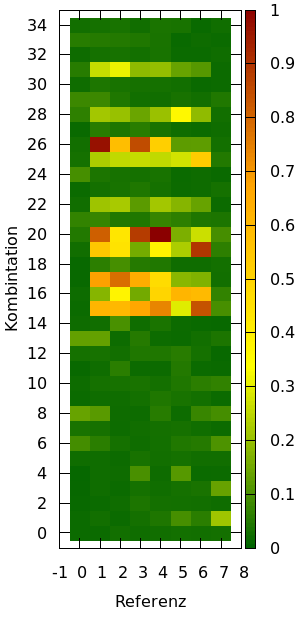
\includegraphics[width=\textwidth]{common/img/ConditionPlot_scaled.png}
                 \caption{Farbkodierte Matrix der Kondition aller möglichen Kombinationen (skaliert auf den höchsten vorkommenden Wert)\\
                 B=> grün~:=~gute -, rot=~schlechte Konditionierung}
                 \label{fig:ConditionMatrix}\textit{}
         \end{subfigure}
%         
\qquad
         \begin{subfigure}[t]{0.4\textwidth}
                 \centering
                 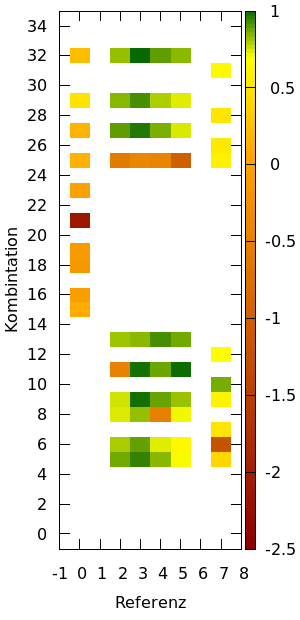
\includegraphics[width=\textwidth]{common/img/60_Results_scaled.png}
                 \caption{ Dargestellt ist Übereinstimmung mit dem wahren Wert, anders ausgedrückt nimmt die Abweichung von oben nach unten zu; Die Position des Ergebnisses in der Matrix entspricht der in der Konditionsmatrix }
                 \label{fig:Results}
         \end{subfigure}
%
\end{figure}


%----------------------------------------------------------------------------
%----------------------------------------------------------------------------
%----------------------------------------------------------------------------
\newpage
\begin{landscape}
	\section{Projektlaufplan KW 26}
	\label{sec:projectplan}
	\scalebox{.75}{
		\begin{ganttchart}[vgrid={draw=none,*1{gray, dashed}},
				hgrid=true,
				today=22,
				title height=1,
				y unit title=0.6cm,
				y unit chart=0.8cm,
				group right shift=0,
				group top shift=.3,
				group height=.3,
				milestone width=.8,
				group peaks={}{}{.2},
				incomplete/.style={fill=black!15}, %
				bar/.style={fill=white}, %
				today label={Heute},
				today rule/.style={dashed, thick}]{44}


\gantttitle{\textbf{2013}}{44} \\
\gantttitlelist{16,...,37}{2} \\
%-------------------------------------------------------------
\ganttgroup{Projekt Evaluation}{3}{14} \\
\ganttbar[progress=100, progress label font=\small\color{black!75},
	progress label anchor/.style={right=4pt}]{Installation der Umgebungen}{3}{6} \\
	
\ganttbar[progress=100, progress label font=\small\color{black!75},
	progress label anchor/.style={right=4pt},
	bar label font=\normalsize\color{black},
	name=rech]{Recherche}{3}{7} \\
	
\ganttmilestone[name=ms1]{Vorstellung der Ergebnisse}{7} \\
	
\ganttbar[progress=90, progress label font=\small\color{black!75},
	progress label anchor/.style={right=4pt},
	bar label font=\normalsize\color{black},
	name=pflichten]
	{Pflichtenheft}{5}{8} \\
	
\ganttmilestone[name=ms2]{Pflichtenheft fertig}{8} \\

\ganttbar[progress=90, progress label font=\small\color{black!75},
	progress label anchor/.style={right=4pt},
	bar label font=\normalsize\color{black},
	name=bNumVerf]
	{Einarbeitung num. Verfahren}{5}{16} \\

\ganttbar[progress=50, progress label font=\small\color{black!75},
	progress label anchor/.style={right=34pt},
	bar label font=\normalsize\color{black},
	name=bCMAES]
	{speziell CMA-ES}{7}{10} \\

\ganttmilestone[name=ms3]{Beurteilung num. Verfahren}{16} \\

\ganttlinkedbar[progress=10, progress label font=\small\color{black!75},
	progress label anchor/.style={right=34pt},
	bar label font=\normalsize\color{black}]
	{Shark Einarbeitung}{17}{18} \\

\ganttlinkedmilestone[name=ms7]{Abschluss Evaluation}{18} \\
	
%-------------------------------------------------------------
\ganttgroup{Erstellung Prototyp}{15}{26} \\
\ganttgroup{(optional)}{15}{18} \\
\ganttbar[progress=25, progress label font=\small\color{black!75},
	progress label anchor/.style={right=4pt},
	bar label font=\normalsize\color{black}]
	{(Entwurf digi. Filter)}{15}{15} \\

\ganttlinkedbar[progress=10, progress label font=\small\color{black!75},
	progress label anchor/.style={right=4pt},
	bar label font=\normalsize\color{black},
	name=bImpFPGA]
	{(Implementation FPGA)}{16}{18} \\

\ganttmilestone[name=ms4]{(Verifikation dig. Filter)}{18} \\
	
\ganttbar[progress=40, progress label font=\small\color{black!75},
	progress label anchor/.style={right=4pt},
	bar label font=\normalsize\color{black},
	name=bImplAlgo]
	{Implementation Algorithmus}{15}{26} \\

\ganttlinkedmilestone[name=ms5]{Implementation Done}{26} \\

%-------------------------------------------------------------
\ganttgroup{Verifikation}{27}{34} \\
\ganttbar[progress=10, progress label font=\small\color{black!75},
	progress label anchor/.style={right=4pt},
	bar label font=\normalsize\color{black},
	name=bVerf]
	{Durchf\"uhrung Verifikation}{27}{34} \\

\ganttlinkedmilestone[name=ms6]{Verifikation Done}{34} \\

%-------------------------------------------------------------
\ganttgroup{Projektdokumentation}{35}{42} \\

\ganttbar[progress=0, progress label font=\small\color{black!75},
	progress label anchor/.style={right=4pt},
	bar label font=\normalsize\color{black},
	name=thesis]
	{Thesis schreiben}{35}{42} \\
	
\ganttmilestone[name=msthesis,milestone label font=\color{red}, 
	milestone/.style={fill=red}]{Abgabe}{42}

%\ganttlink{ms7}{bImplAlgo}
\ganttlink{bImpFPGA}{ms4}
\ganttlink{bNumVerf}{ms3}
\ganttlink{bCMAES}{ms3}
\ganttlink{rech}{ms1}
\ganttlink{pflichten}{ms2}
\ganttlink{thesis}{msthesis}

	\end{ganttchart}
		}
\end{landscape}

%----------------------------------------------------------------------------

\end{appendix}


\newpage
%- Bibliography --------------------------------------------------------------
\bibliographystyle{ieeetr}
\bibliography{../bib/mathesis_collection1}

\end{document}